% \documentclass{beamer}
%\documentclass[handout]{beamer}
%\usepackage{pgfpages} \pgfpagesuselayout{4 on 1}[a4paper,landscape,border shrink=2mm]

\documentclass[aspectratio=169]{beamer}
%\documentclass[aspectratio=169,handout]{beamer}
%\usepackage{pgfpages} \pgfpagesuselayout{4 on 1}[a4paper,landscape,border shrink=2mm]

\usepackage{ESE_beamer}

\title{Presentation title}
\subtitle{Sub-title}
\author{Author}
\date{\today}
\footer{Erasmus School of Economics}	% Comment out for no footer

%\noyellowtitle							% Remove yellow title bars (matches new 'official' style)
%\dropframenumbers						% Hide frame numbers
% \nocopyright							% Completely remove copyright notice
%\setcopyright{Don't use this!}

\begin{document}
\titlepage % Use for title page without picture

% \titlepagePicture{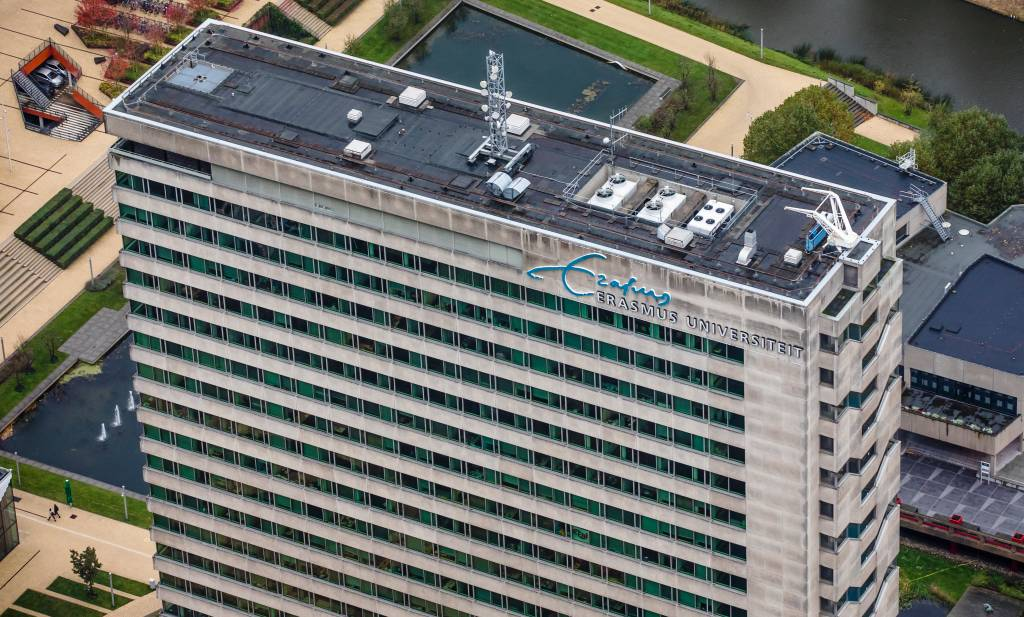
\includegraphics[height=9cm,trim=3cm 2.5cm 0cm 0cm, clip=true]{erasmusPhoto.jpeg}} %for aspectratio=16x9: picture should be 16x9cm at least

% \titlepagePicture{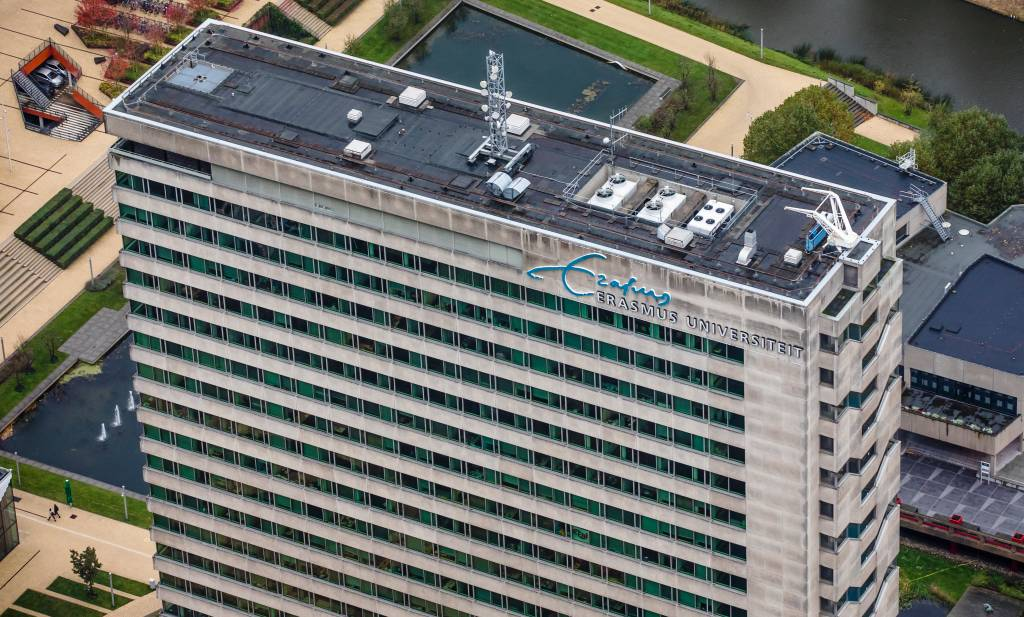
\includegraphics[height=9.6cm]{erasmusPhoto.jpeg}} %for aspectratio=4x3: picture should be 12.9x9.6cm at least)

% \titlepagePictureWithBorder{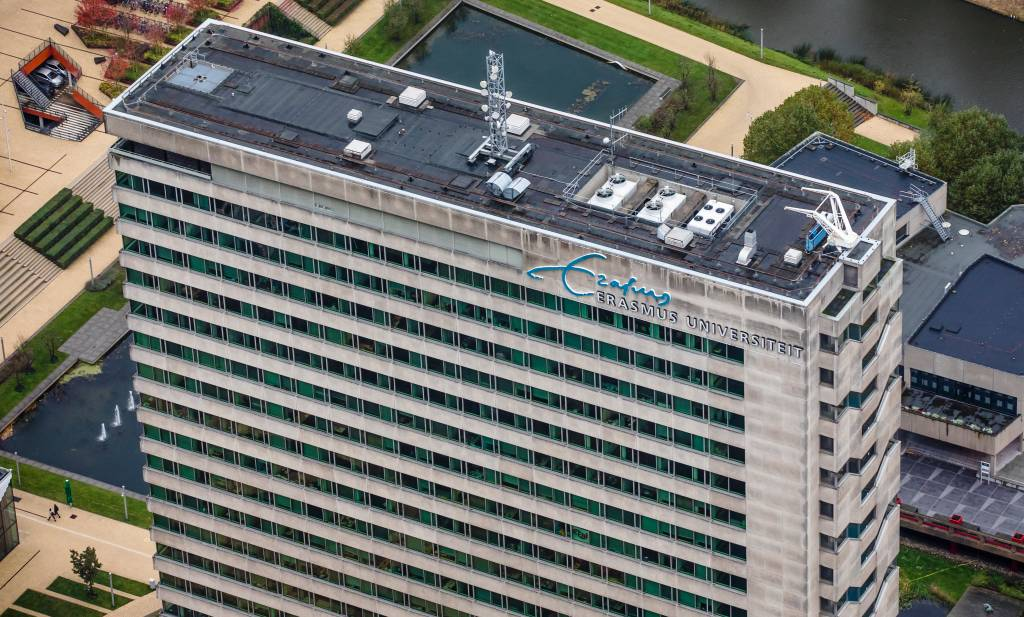
\includegraphics[height=9cm,trim=3cm 2.5cm 0cm 0cm, clip=true]{erasmusPhoto.jpeg}} %for aspectratio=16x9: picture should be 16x9cm at least

\begin{frame}{Example slide}
\begin{itemize}
	\item The EUR copyright notice is included by default
	\item $\backslash$nocopyright completely removes copyright statement
	\item $\backslash$setcopyright\{text\} sets the copyright line to ``text'' (can be empty)
	\item {\tt $\backslash$documentclass[]\{beamer\}} gives $4\times3$ aspectratio
	\item {\tt $\backslash$documentclass[aspectratio=169]\{beamer\}} gives $16\times9$ aspectratio	
\end{itemize}

\end{frame}

\begin{frame}{Example slide}\thispagestyle{empty}
	A slide without logo and page number.
\end{frame}

\breakframe{A new topic ($\backslash$breakframe\{\})}

\fancybreakframe{A new topic ($\backslash$fancybreakframe\{\})}

\begin{frame}{Itemize and enumerate layout}
\begin{itemize}
	\item Default bullets
	\begin{itemize}
		\item are blue
	\end{itemize}
\end{itemize}
and
\begin{enumerate}
	\item Enumerations 
	\begin{enumerate}
		\item are blue as well
	\end{enumerate}
\end{enumerate}
Command \texttt{$\backslash$yellowItemize} changes this
\yellowItemize
\begin{itemize}
	\item Default bullets
	\begin{itemize}
		\item are now yellow
	\end{itemize}
\end{itemize}
and 
\begin{enumerate}
	\item Enumerations 
	\begin{enumerate}
		\item are yellow as well
	\end{enumerate}
\end{enumerate}

\end{frame}
\end{document}